\subsection{HTML5 and CSS3} % (fold)
\label{sub:html5css3}

\ida{HTML} 5 is the next generation of \ida{HTML}, and it includes a lot of new functionality\cite{HTML5NEW}.
Unlike its predecessors, it is not a great big monolithic specification.
Indeed, the term \ida{HTML} 5 encompasses the latest round of web standards and specifications, including \ida{HTML} 5 itself, \ida{CSS} 3 and other extensions that define additional \idas{API}s for \ida{HTML} documents.

Since it is mostly backwards compatible, it can be reasonably used today.
Those browsers which supports that part of the specification should work fully or partially, while the rest should fallback to an acceptable rendering.
The important thing is that, even if the specification is not finished, a web application can choose to use a slice of it to enhance the user experience.

One focus of \ida{HTML} 5 is to improve the structure of a document by adding new semantic elements, primarily to avoid the \idc{div} soup.
Figure~\vref{fig:html-structure} introduces the new \idc{article}, \idc{aside}, \idc{header}, \idc{footer} and \idc{nav} elements and compares it with the traditional \ida{HTML} 4 approach.
At the same time, a lot of non-semantical elements have been deprecated.

\begin{figure}[htbp]
  \centering
  \subfigure[HTML 4 Structure]{
    \label{fig:html4-structure}
    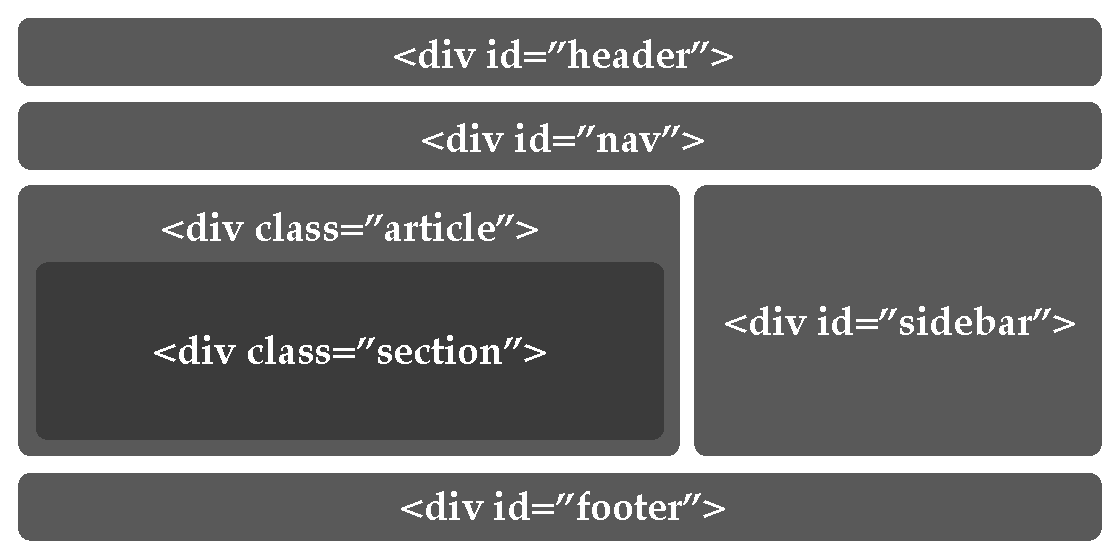
\includegraphics[width=\textwidth]{html4-structure}
  }
  \subfigure[HTML 5 Structure]{
    \label{fig:html5-structure}
    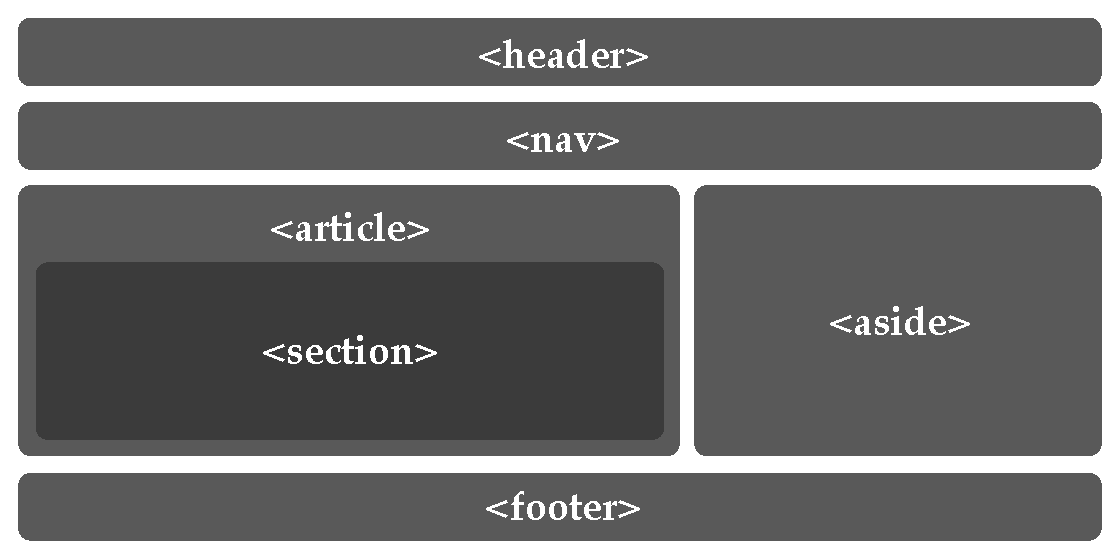
\includegraphics[width=\textwidth]{html5-structure}
  }
  \caption{Structure of typical HTML 4 and HTML 5 documents}
  \label{fig:html-structure}
\end{figure}

But probably the most popular new feature in \ida{HTML} 5 is the new built-in multimedia integration.
By using the new \idc{video} and \idc{audio} elements, a browser can play natively video and audio files.
And with the \idc{canvas} element a page can draw anything in a page.
These additions make proprietary plugins dispensable in most scenarios, such as Adobe \idx{Flash}, Microsoft Silverlight or \idx{Java applet}s.

A lot of new attributes have been added and, in some occasions, deprecated.
Forms have got a well-received update with more specific input elements (to write an email or an \ida{URL}, to choose a date or a color, etc.) with auto-validation capabilities.
All elements can be \emph{draggable} or \emph{editable} with the flip of an attribute.

Additional modules to the main specification give web applications the ability to store information in the browser in a local database (see \S~\vref{ssub:domobjects}) and caching resources, allowing the development of offline web applications.
Other modules give new \idas{API}s to manipulate and process local files right in the browser, with no need of sending it to the server.

Files from the computer can be dropped in the browser (in mass or individually) so the web application can read them directly, and files with a certain \ida{MIME} type can also be linked to a specific web application.
For example, images can be configured to be open by default in a web image editor, instead of with a local application.

Another possibility is to directly manipulate the history of the browser, very useful for \ida{AJAX}-based applications.
Other new features are geo-localization (to know where the user is physically located), notifications (to notify events in the browser) and Web Sockets (to open a socket right from the browser).

Given the huge web applications that can be developed on top of these new features, performance could become critical very quickly.
Web Workers are available to run heavy tasks in the background in parallel with the main loop.
If \idx{JavaScript} code is too inefficient for the task, there is an \ida{HTML} 5 extension to run compile native code (written in C/C++).
Even with the use of \ida{WEBGL}, the development of interactive native 3D applications is possible.

Many, if not all of these new capabilities, are closely linked with the use of \idx{JavaScript}.
There is an \ida{API} for every feature, to modify the state and integrate it with the web application.
Additional discussion over the \ida{DOM} takes place in \S\vref{sub:dom}.

On the other hand, \ida{CSS} 3 is also considered to be a big step in web development.
In order to speed up the tedious standardization process, the \ida{CSS} 3 specification effort is much more modular than the \ida{HTML} 5 specification.
Currently there are more than 50 micro-specifications in work, with uneven progress.
Some of the most important new features are:

\begin{description}
  \item[Media queries] Now media queries are more important than before, allowing device targeting.
  For example, some rules or stylesheets can be specifically designed to only affect a mobile device when it is oriented in portrait, or a generic device when it has more than 960 pixels of width.
  \item[Selectors] New selectors are introduced, mostly to target dynamic pseudo elements.
  Two new pseudo selectors, \idc{::before} and \idc{::after}, are more special, because they generated new visual elements in the page, very useful to recreate artifacts.
  \item[Borders] In \ida{CSS} 3 borders are incredibly powerful: it can have rounded corners with different radius for each corner, and images can be used to fill the border no matter the size of the box.
  \item[Shadows] There are two kind of shadows: box shadows and text shadows.
  Box shadows are applied to the elements boxes, while text shadows are applied to the text itself.
  Both shadows can be either inner or outer, and they have to specify a color, opacity, direction, size and blur.
  A shadow value can be composed by a undetermined number of shadows.
  \item[Gradients] For backgrounds, borders or any property that accepts an image, a gradient color can be generated on the fly by the browser.
  A gradient can be composed by any number of color stops, it supports opacity changes and it can be either linear or radial.
  \item[Multiple Backgrounds] Going further, backgrounds can be dynamically composed with several images, gradients and colors.
  This is very useful when the sources have opacity, since it allows complex compositions, e.g., mixing textures and several shadows.
  \item[Transforms] An element can be easily rotated, skewed, translated or scaled.
  Additional 3D transformations are defined in another \ida{CSS} module, with the same transformations in 3D and a perspective function.
  \item[Transitions] \ida{CSS} 3 allows to gracefully transition an element from a state to another, for example when the class is changed or when the mouse is hovering the element.
  In those cases two different declaration blocks are defined for each class (or pseudo-class), and instead of a sharp change of values the element will slowly morph into the new values.
  To set a transition it is needed to specify the altered properties (or all), the timing function (the speed curve of the transition effect) and the total time to spent in the effect.
  \item[Animations] Similar to transitions, an element can be animated using only \ida{CSS} rules.
  Two or more keyframes need to be defined, with the set of properties and values that the element will take each keyframe.
  Then, according to its parameters (duration, timing function and iteration count), the styles are smoothly interpolated from keyframe to keyframe.
  \item[Web Fonts] Although the \idc{@font-face} rule was introduced in \ida{IE}4 (1997), until recently the use of custom fonts in web pages was not widespread.
  One of the reasons is that there is no single format compatible with all major browsers.
  Even now, to target the maximum number of browsers five different files have to be deployed, each with a different font format.
  In the near future the \ida{WOFF} is supposed to be the standard, simplifying this process.
\end{description}

When a browser implements some of those properties, since most of these modules are a work in progress or directly they were proposed by that browser, their names are usually preceded by a vendor prefix.
For example, \idc{border-radius} was called \idc{-webkit-border-radius} in \idx{Webkit} browsers, \idc{-moz-border-radius} in \idx{Firefox} and \idc{-o-border-radius} in \idx{Opera}.
Later, when the standard was more settled, they all changed it to \idc{border-radius}.
For this reason any modern web application that wants to use such a modern property now have to specify redundant rules targeting each browser engine.

% subsection html5css3 (end)